\chapter{Polarization of single top quarks in \textsl{t}~channel at 8~TeV}

\intro{A first measurement of the top quark spin asymmetry in t~channel, related to the top quark polarization, is presented in this chapter. Proton-proton collision data at $\mathit{\sqrt{s}=8}$~TeV have been analyzed corresponding to about $\mathit{20~fb^{-1}}$. Events with an isolated muon are selected together with two or three jets for the final measurement while events containing an isolated electron and jets have been studied as well. The normalized differential cross section is measured as a function of the polarization angle. From its shape, a spin asymmetry of $\mathit{0.26\pm0.03~(stat)\pm0.10~(syst)}$ is obtained. This is found to be compatible within $\mathit{2.0}$ standard deviations with the expected \gls{sm} asymmetry of $\mathit{0.44}$. The result has been published in Ref.~\cite{Khachatryan:2015dzz}. In a further step, the derivation of limits on anomalous couplings is illustrated by combining this measurement with related ones.}


An overview of the strategy to measure the top quark spin asymmetry and derive limits on anomalous couplings is given in the following. After selecting events with an isolated muon or electron and two or three jets, two \glspl{bdt} are employed. The first one, \bdtqcd, is trained to reject events with fake leptons stemming from multijet production. The amount of multijet contamination after the event selection is estimated through a two-component \gls{ml} fit to the \bdtqcd discriminant where other contributions from signal and background processes are kept together. The multijet background is modeled by a template obtained from data in a sideband region for which the lepton isolation is inverted. The second \gls{bdt}, \bdttch, is optimized to separate signal from \wjets and \ttbar events. The amount of signal and background fractions is estimate through a second \gls{ml} fit to its discriminant. A signal-enhanced phase space is obtained by applying an optimized selection on each of the \glspl{bdt} discriminants resulting in a \gls{sb} ratio of about 90\%. The shape of the polarization angle, $\cos\theta^\star_{\mu}$, in data is unfolded to parton level after subtracting the remaining background contributions. This is repeated for each considered source of systematic uncertainty to estimate their impact on the measurement. The final measurement is performed in the muon channel only since in the electron channel, shortcomings in the modeling of the data-driven multijet template and an overall larger impact of systematic uncertainties are observed rendering its standalone result much less significant. From the differential cross section the asymmetry is obtained by a linear fit while accounting for the induced bin-by-bin correlations from the unfolding. The \TOPFIT program is utilized in a further step to derive limits on anomalous Wtb couplings by combining the measured asymmetry with an inclusive cross section measurement in $t$~channel and a measurement of the W~boson helicity fractions in \ttbar production.



%##############################################
\section{Event selection and simulated samples}
%##############################################

Proton-proton collision data at $\sqrt{s}=8~\TeV$ are analyzed corresponding to $19.7~\invfb$ recorded with the \gls{cms} experiment in 2012. Events are triggered on the presence of a single muon or electron candidate. The employed single muon trigger requires isolated muon candidates with $\pt>24~\GeV$ which fall within the pseudorapidity range of $|\eta|<2.1$. The single electron trigger fires when an electron candidate with $\pt>27~\GeV$ within $|\eta|<2.5$ is detected which has to fulfill some quality criteria in addition corresponding to an efficiency of 80\% for prompt electrons. Motivated by the decay mode of the W~boson under the signal hypothesis, the events are categorized into ``channels'' depending if they have been triggered with the muon or electron trigger. In the analysis, events in the muon channel have to contain one muon candidate with $\pt>26~\GeV$ within $|\eta|<2.1$ that passes the tight identification requirements. In the electron channel, events considered for analysis have to contain one electron candidate with $\pt>30~\GeV$ within $|\eta|<2.5$ that fulfills the tight \gls{mva}-based  identification. To suppress fake leptons from multijet production, the muon candidate has to have a relative \gls{deltabeta}-based isolation of $\muiso<12\%$ while the electron candidate has to have a relative \gls{effarea}-based isolation of $\eiso<10\%$. Events containing additional muons~($\pt>10~\GeV$, $|\eta|<2.5$) or electrons~($\pt>20~\GeV$, $|\eta|<2.5$) which pass corresponding loose identification criteria are rejected to suppress contributions from \zjets and dileptonic \ttbar production. 

Jets are clustered from \gls{pf} candidates with the anti-\kt algorithm using a distance parameter of $R=0.5$ while applying the \gls{chs} technique to remove the contamination of pileup tracks. \gls{pf} candidates belonging to preselected loosely isolated muons are not clustered into the jets to prevent double counting. In addition, jets which are within $\Delta R<0.3$ to the previous selected tight lepton are ignored in the analysis. The reconstructed jet energy in data and simulation and the energy resolution in simulation are calibrated through dedicated \gls{jec} and \gls{jer} scale factors. Events containing two or three jets with $\pt>40~\GeV$ that are detected within $|\eta|<4.5$ and pass loss identification criteria are considered for analysis. Tagging of jets which likely originated from the hadronization of a b~quark is performed with the \gls{csv} algorithm. Such jets are restricted to $|\eta|<2.4$ since the b-tagging algorithm operates only within the acceptance of the inner tracking system. An efficiency of about 50\% for tagging true b~jets with a mistagging rate of 0.1\% for other jets is found in simulation using the tight b-tagging working point. The b-tagging efficiency is reweighted in simulation through scale factors to match the one measured in data. More details about the employed analysis objects, identification, and corrections are described in Ch.~\ref{ch:reconstruction}.

Events are categorized as shown in Fig.~\ref{fig:polarization-categorization}. The different regions are labeled as ``$N\,\mathrm{j}~M\,\mathrm{t}$'' where $N$ denotes the number of selected jets and $M$ the subset of jets which are also b-tagged. Control regions dominated by either \wjets~(2j0t) or \ttbar~(3j1t, 3j2t) production are defined besides the signal region~(2j1t). The analysis was developed by validating the background modeling and optimizing the strategy by comparing to data in the control regions only. During this process, data in the signal region has not been used. This procedure is commonly referred to as ``blinding''. After the strategy is fixed the final measurement is conducted by unblinding the signal region while refraining from any further optimizations. The blinding procedure prevents a result-driven tuning of the analysis strategy which could bias the measurement.

\myfigure{\label{fig:polarization-categorization}Categorization of events depending on number of selected jets, number of b-tags, and the signal \gls{bdt} discriminant. The shaded regions are utilized in a template-based \gls{ml} fit as described in Sec.~\ref{sec:polarization-fit} for estimating the signal and background yields.}{
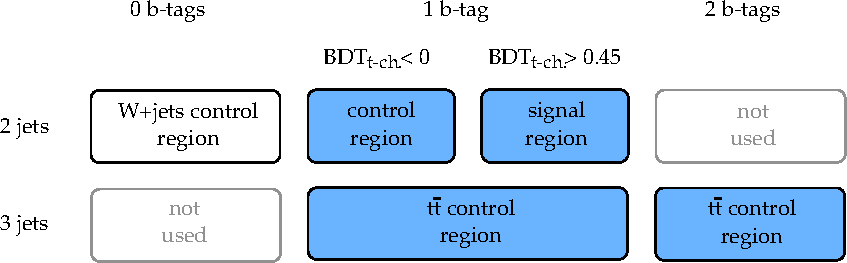
\includegraphics[scale=0.75]{figures/polarization/regions.pdf}
}

Various samples of simulated events for signal and background processes are generated. The default signal sample is generated in 5~\gls{fs} using the \POWHEG\,v1 generator interfaced with \PYTHIA\,6 for parton showering and \TAUOLA for tau decays. For comparisons, two additional, alternative signal samples are generated. One utilizes the \AMC generator interfaced with \PYTHIA\,8 in 4~\gls{fs} while the other employs the \COMPHEP generator interfaced with \PYTHIA\,6. A set of special samples with anomalous Wtb couplings is generated as well using the \COMPHEP generator for testing the analysis strategy. Samples containing single top quark events produced via tW and $s$~channel are generated with \POWHEG\,v1 interfaced with \PYTHIA\,6 and \TAUOLA. The major background processes, \wjets, \zjets, and \ttbar, are generated with the \MG generator interfaced with \PYTHIA\,6 and \TAUOLA as well. Samples with up to three~(\ttbar) or four~(\wjets,\zjets) additional partons at \gls{me} level are merged together using the \gls{mlm} merging procedure. For \wjets production, an alternative sample generated with \SHERPA~\cite{Hoeche:2012ft} is employed for validation purposes. In this thesis, \wjets events are categorized based on their jet flavor content. Events with at least one heavy-quark flavored jet from either c, or b~quarks are referred to as ``\gls[]{whf}'' while events with only light-quark flavored jets~(g,u,d,s) are labeled as ``\gls[]{wlf}'' instead. Diboson production~(WW,WZ,ZZ) is a minor background and simulated with \PYTHIA\,6. The cross sections used to normalize the samples are listed in Tab.~\ref{tab:polarization-theo-xsecs}.


\mytable{\label{tab:polarization-theo-xsecs}Theoretical cross sections used to normalize the simulated samples.}{
\begin{tabular}{|l  r c l |}
\hline
process & $\sigma/\pb$ &\hspace{0.1cm} & accuracy \\
\hline
$t$~channel & $87.1~\pb$ & & approx. \gls{nnlo}~\cite{Kidonakis:2012db} \\
$s$~channel & $5.55~\pb$ && approx. \gls{nnlo}~\cite{Kidonakis:2012db}  \\
tW~channel & $22.2~\pb$ && approx. \gls{nnlo}~\cite{Kidonakis:2012db} \\
\ttbar & $252.9~\pb$ && \gls{nnlo} (using Top++\,2.0~\cite{Czakon:2011xx}) \\
$\mathrm{W}\to\ell\nu\mathrm{\,\mbox{+}\,jets}$ & $37\,509~\pb$ && \gls{nnlo} (using FEWZ~\cite{Gavin:2010az}) \\
$\mathrm{Z}/\gamma^{*}\to\ell^{\rmplus}\ell^{\rmminus}$, $m_{\ell\ell}>50~\GeV$ & $3\,504~\pb$ && \gls{nnlo} (using FEWZ~\cite{Gavin:2010az}) \\
WW & $54.8~\pb$ && \gls{nlo} (using MCFM\,5.8~\cite{Campbell:2010ff})\\
WZ & $33.2~\pb$ && \gls{nlo} (using MCFM\,5.8~\cite{Campbell:2010ff})\\
ZZ & $8.1~\pb$ && \gls{nlo} (using MCFM\,5.8~\cite{Campbell:2010ff})\\
\hline
\end{tabular}
}

The fake muon background stemming from multijet production is estimated from a data sideband region. For this the lepton isolation requirement is inverted. The distribution of data serves as a template of the shape of multijet production after subtracting the remaining contamination by other processes. Figure~\ref{fig:polarization-qcd-template} shows the distribution of the transverse W~boson mass in this sideband region and the resulting multijet template after it has been fitted to data in the 2j1t signal+control region. The extracted template yields a good description of the unknown multijet shape in the signal region after the fit.

\myfigure{\label{fig:polarization-qcd-template}Distributions of the transverse W~boson mass in muon channel: (a)~antiisolated sideband region for extracting the multijet template; (b)~resulting distribution in the 2j1t region after scaling the extracted template to data through a \gls{ml} fit.}{
\subfloat[]{\adjincludegraphics[height=4.8cm,trim={0 0 {0.23\width} 0},clip]{figures/polarization/beforeBgCorr/2j1t/muon_2j1t_mtw_qcdnone_antiiso_nol.pdf}}\hspace{0.017\textwidth}
\subfloat[]{\adjincludegraphics[height=4.8cm,trim={0 0 {0.\width} 0},clip]{figures/polarization/beforeBgCorr/2j1t/muon_2j1t_mtw_qcdnone.pdf}}
}


Distributions of the reconstructed top quark mass in muon and electron channel after the event selection are shown in Fig.~\ref{fig:polarization-topmass}. In control regions containing no or more than one b-tagged jet, the jet with the highest value of the \gls{csv} discriminant is associated to the top quark decay to calculate the top quark mass. The individual signal and background templates have been scaled to the result of a binned \gls{ml} fit to data here and elsewhere in this chapter unless otherwise stated. The presented plots display a fair agreement with data.




\myfigure{\label{fig:polarization-topmass} Distributions of the reconstructed top quark mass in (left column)~electron and (right column)~muon channel. Top row: 2j0t \wjets control region; middle row: 2j1t region; bottom row: 3j1t \ttbar control region.}{
\subfloat[]{\adjincludegraphics[height=4.8cm,trim={0 0 {0.23\width} 0},clip]{figures/polarization/beforeBgCorr/2j0t/electron_2j0t_top_mass_qcdnone_nol.pdf}}\hspace{0.017\textwidth}
\subfloat[]{\adjincludegraphics[height=4.8cm,trim={0 0 {0.\width} 0},clip]{figures/polarization/beforeBgCorr/2j0t/muon_2j0t_top_mass_qcdnone.pdf}}\\
\subfloat[]{\adjincludegraphics[height=4.8cm,trim={0 0 {0.23\width} 0},clip]{figures/polarization/beforeBgCorr/2j1t/electron_2j1t_top_mass_qcdnone_nol.pdf}}\hspace{0.017\textwidth}
\subfloat[]{\adjincludegraphics[height=4.8cm,trim={0 0 {0.\width} 0},clip]{figures/polarization/beforeBgCorr/2j1t/muon_2j1t_top_mass_qcdnone.pdf}}\\
\subfloat[]{\adjincludegraphics[height=4.8cm,trim={0 0 {0.23\width} 0},clip]{figures/polarization/beforeBgCorr/3j2t/electron_3j2t_top_mass_qcdnone_nol.pdf}}\hspace{0.017\textwidth}
\subfloat[]{\adjincludegraphics[height=4.8cm,trim={0 0 {0.\width} 0},clip]{figures/polarization/beforeBgCorr/3j2t/muon_3j2t_top_mass_qcdnone.pdf}}
}


\clearpage

%##############################################
\section{Training of Boosted Decision Trees}
%##############################################
\label{sec:polarization-bdt-training}

Two \glspl{bdt} are trained to obtain a signal enhanced phase space. The first \gls{bdt}, labeled \bdtqcd, is trained to reject background events stemming from multijet production. 


The following observables are chosen as input for the training:
\begin{itemize}
\item the missing transverse energy, \met;
\item the reconstructed mass of the top quark candidate;
\item the transverse mass of the W~boson candidate, \mtw, before solving for the unknown neutrino $p_{z}$ component since this modifies \pvmiss in case of complex solutions;
\item the event isotropy which is defined as $(s_\mathrm{max}-s_\mathrm{min})/s_\mathrm{max}$ with $s=\sum_{i}^\scriptn{\ell,\,\mathrm{jets}}\big|\,\vec{n}\cdot\vec{p}_{i}\big|$ where the unit vector $\vec{n}=(\cos\phi,\sin\phi)$ is chosen in the transverse plane to either maximize or minimize $s$.
\end{itemize}


The \bdttch discriminant is trained using the following observables as input:
\begin{itemize}
\item the reconstructed mass of the top quark candidate;
\item the absolute pseudorapidity of the untagged spectator jet, ``$\jprime~|\eta|$''\,;
\item the absolute pseudorapidity of the b-tagged jet, ``$\mathrm{b~jet}~|\eta|$''\,;
\item the mass of the b-tagged jet from the summed momenta of the clustered \gls{pf} candidates;
\item the transverse momentum of the muon;
\item the transverse momentum of the b-tagged jet;
\item the missing transverse energy, \met;
\item the mass of the top quark and the spectator jet system, $\sqrt{\hat{s}}=\big|\vec{p}_{\mathrm{top}}+\vec{p}_{\jprime}\big|$\,;
\item the transverse momentum of the hadronic final-state system, ``$\mathrm{\gls[]{hfs}}~\pt$''\,=~$\big(\vec{p}_{\jprime}+\vec{p}_{\mathrm{b}}\big)_\mathrm{T}$\,.
\end{itemize}

\myfigure{\label{fig:polarization-event-observables}Distributions of ???.}{
\subfloat[]{\adjincludegraphics[height=4.8cm,trim={0 0 {0.23\width} 0},clip]{figures/polarization/beforeBgCorr/2j1t/muon_2j1t_ljet_pt_qcdnone_nol.pdf}}
\hspace{0.017\textwidth}
\subfloat[]{\adjincludegraphics[height=4.8cm]{figures/polarization/beforeBgCorr/2j1t/muon_2j1t_ljet_abseta_qcdnone.pdf}}\\
\subfloat[]{\adjincludegraphics[height=4.8cm,trim={0 0 {0.23\width} 0},clip]{figures/polarization/beforeBgCorr/2j1t/muon_2j1t_isotropy_qcdnone_nol.pdf}}
\hspace{0.017\textwidth}
\subfloat[]{\adjincludegraphics[height=4.8cm,trim={0 0 {0.\width} 0},clip]{figures/polarization/beforeBgCorr/2j1t/muon_2j1t_bjet_mass_qcdnone.pdf}}
\hspace{0.017\textwidth}\\
\subfloat[]{\adjincludegraphics[height=4.8cm,trim={0 0 {0.23\width} 0},clip]{figures/polarization/beforeBgCorr/2j1t/muon_2j1t_shat_logmass_qcdnone_nol.pdf}}
\hspace{0.017\textwidth}
\subfloat[]{\adjincludegraphics[height=4.8cm]{figures/polarization/beforeBgCorr/2j1t/muon_2j1t_hfs_logpt_qcdnone.pdf}}
}


\myfigure{\label{fig:polarization-bdts}Distributions of ???.}{
\subfloat[]{\adjincludegraphics[height=4.8cm,trim={0 0 {0.23\width} 0},clip]{figures/polarization/beforeBgCorr/2j1t/muon_2j1t_bdt_qcd_qcdnone_nol.pdf}}
\hspace{0.017\textwidth}
\subfloat[]{\adjincludegraphics[height=4.8cm]{figures/polarization/beforeBgCorr/2j1t/muon_2j1t_bdt_tch_qcdnone.pdf}}
}

choice of variables, correlation tests



%##############################################
\section{Background modeling}
%##############################################
wjets: flavor, cosTheta (sherpa)
ttbar: top pt -> modifies mass

\myfigure{\label{fig:polarization-wjets-reweighting}Distributions of ???.}{
\subfloat[]{\adjincludegraphics[height=4.8cm,trim={0 0 {0.23\width} 0},clip]{figures/polarization/beforeBgCorr/2j0t/muon_2j0t_cosTheta_lj_qcdbdt_nol.pdf}}
\hspace{0.017\textwidth}
\subfloat[]{\adjincludegraphics[height=4.8cm,trim={0 0 {0.\width} 0},clip]{figures/polarization/afterBgCorr/2j0t/muon_2j0t_cosTheta_lj_qcdbdt.pdf}}\\
\subfloat[]{\adjincludegraphics[height=4.8cm,trim={0 0 {0.23\width} 0},clip]{figures/polarization/beforeBgCorr/2j0t/muon_2j0t_wboson_pt_qcdbdt_nol.pdf}}
\hspace{0.017\textwidth}
\subfloat[]{\adjincludegraphics[height=4.8cm,trim={0 0 {0.\width} 0},clip]{figures/polarization/afterBgCorr/2j0t/muon_2j0t_wboson_pt_qcdbdt.pdf}}
}

\myfigure{\label{fig:polarization-toppt-reweighting}Distributions of the transverse momentum of the reconstructed top quark in 3j1t control region (a)~before and (b)~after applying the top quark $\pt$ reweighting.}{
\subfloat[]{\adjincludegraphics[height=4.8cm,trim={0 0 {0.23\width} 0},clip]{figures/polarization/beforeBgCorr/3j2t/muon_3j2t_top_logpt_qcdbdt_nol.pdf}}
\hspace{0.017\textwidth}
\subfloat[]{\adjincludegraphics[height=4.8cm]{figures/polarization/afterBgCorr/3j2t/muon_3j2t_top_logpt_qcdbdt.pdf}}
}


\myfigure{\label{fig:polarization-dphi-lepton-met}Distributions of the angle in the transverse plane between the missing transverse momentum and the (a)~muon, (b)~electron after applying the described corrections.}{
\subfloat[]{\adjincludegraphics[height=4.8cm,trim={0 0 {0.23\width} 0},clip]{figures/polarization/afterBgCorr/2j0t/electron_2j0t_lepton_met_dphi_qcdnone_nol.pdf}}
\hspace{0.017\textwidth}
\subfloat[]{\adjincludegraphics[height=4.8cm]{figures/polarization/afterBgCorr/2j0t/muon_2j0t_lepton_met_dphi_qcdnone.pdf}}
}

%##############################################
\section{Signal extraction}
%##############################################
\label{sec:polarization-fit}

ml fit;

2j0t excluded from fit since it contains only W+LF
3j2t best for ttbar handle since no multijet


%##############################################
\section{Validation}
%##############################################

\myfigure{\label{fig:polarization-cosTheta-CR}.}{
\subfloat[]{\adjincludegraphics[height=4.8cm,trim={0 0 {0.23\width} 0},clip]{figures/polarization/afterBgCorr/2j1t/muon_2j1t_cosTheta_lj_CR_nol.pdf}}
\hspace{0.017\textwidth}
\subfloat[]{\adjincludegraphics[height=4.8cm]{figures/polarization/afterBgCorr/3j2t/muon_3j2t_cosTheta_lj_qcdbdt.pdf}}
}

\myfigure{\label{fig:polarization-cosTheta-SR}.}{
\subfloat[]{\adjincludegraphics[height=4.8cm,trim={0 0 {0.23\width} 0},clip]{figures/polarization/afterBgCorr/2j1t/muon_2j1t_cosTheta_lj_SR_nol.pdf}}
\hspace{0.017\textwidth}
\subfloat[]{\adjincludegraphics[height=4.8cm]{figures/polarization/afterBgCorr/2j1t/muon_2j1t_cosTheta_whel_SR.pdf}}
}


cosTheta, cosWhel, top mass in SR/CR, 2j0t,3j1t


%##############################################
\section{Unfolding}
%##############################################

bdt cut, neyman construction, 2bin cross check

\myfigure{\label{fig:polarization-bdtscan}.}{
\adjincludegraphics[height=4.8cm]{figures/polarization/unfolding/scan_mu.pdf}
}

\myfigure{\label{fig:polarization-neyman}.}{
\adjincludegraphics[height=4.8cm]{figures/polarization/unfolding/neyman_t_tbar.pdf}
}



%##############################################
\section{Statistical evaluation}
%##############################################

Q-scale reweighting, chi2 fit

\mytable{}{
\begin{tabular}[htc]{|r | r  r  r |}
\hline 
 
        & $\delta \AmuT\cdot 10^{2}$
        & $\delta \AmuTbar\cdot 10^{2}$
        & $\delta \AmuTplusTbar\cdot 10^{2}$
         \\

\hline 
statistical & $3.2$ \hspace{0.1cm}  & $4.6$ \hspace{0.1cm}  & $2.6$ \hspace{0.1cm}  \\
limited MC & $2.1$ \hspace{0.1cm}  & $3.2$ \hspace{0.1cm}  & $1.8$ \hspace{0.1cm}  \\  
\gls{ml}-fit uncertainty & $0.7$ \hspace{0.1cm}  & $1.2$ \hspace{0.1cm}  & $0.6$ \hspace{0.1cm}  \\ 
Diboson fraction & $<0.1$ \hspace{0.1cm}  & $<0.1$ \hspace{0.1cm}  & $<0.1$ \hspace{0.1cm}  \\ 
\zjets fraction & $<0.1$ \hspace{0.1cm}  & $<0.1$ \hspace{0.1cm}  & $<0.1$ \hspace{0.1cm}  \\ 
$s$~channel fraction & $0.3$ \hspace{0.1cm}  & $0.2$ \hspace{0.1cm}  & $0.2$ \hspace{0.1cm}  \\ 
tW fraction & $0.1$ \hspace{0.1cm}  & $0.7$ \hspace{0.1cm}  & $0.2$ \hspace{0.1cm}  \\ 
multijet shape & $0.5$ \hspace{0.1cm}  & $0.7$ \hspace{0.1cm}  & $0.5$ \hspace{0.1cm}  \\ 
multijet yield & $1.9$ \hspace{0.1cm}  & $1.2$ \hspace{0.1cm}  & $1.7$ \hspace{0.1cm}  \\ 
\hline
b-tagging & $0.7$ \hspace{0.1cm}  & $1.2$ \hspace{0.1cm}  & $0.9$ \hspace{0.1cm}  \\ 
mistagging & $<0.1$ \hspace{0.1cm}  & $0.1$ \hspace{0.1cm}  & $<0.1$ \hspace{0.1cm}  \\ 
\gls{jer} & $2.7$ \hspace{0.1cm}  & $1.8$ \hspace{0.1cm}  & $2.0$ \hspace{0.1cm}  \\ 
\gls{jec} & $1.3$ \hspace{0.1cm}  & $2.6$ \hspace{0.1cm}  & $1.1$ \hspace{0.1cm}  \\ 
unclustered \met & $1.1$ \hspace{0.1cm}  & $3.3$ \hspace{0.1cm}  & $1.3$ \hspace{0.1cm}  \\ 
pileup & $0.3$ \hspace{0.1cm}  & $0.2$ \hspace{0.1cm}  & $0.2$ \hspace{0.1cm}  \\ 
lepton ID & $<0.1$ \hspace{0.1cm}  & $<0.1$ \hspace{0.1cm}  & $<0.1$ \hspace{0.1cm}  \\ 
muon isolation & $<0.1$ \hspace{0.1cm}  & $<0.1$ \hspace{0.1cm}  & $<0.1$ \hspace{0.1cm}  \\ 
trigger efficiency & $<0.1$ \hspace{0.1cm}  & $<0.1$ \hspace{0.1cm}  & $<0.1$ \hspace{0.1cm}  \\ 
\hline
\ttbar top quark \pt reweighting & $0.3$ \hspace{0.1cm}  & $0.3$ \hspace{0.1cm}  & $0.3$ \hspace{0.1cm}  \\ 
\wjets W~boson \pt reweighting & $0.1$ \hspace{0.1cm}  & $0.1$ \hspace{0.1cm}  & $0.1$ \hspace{0.1cm}  \\ 
\wjets heavy flavor fraction & $4.7$ \hspace{0.1cm}  & $6.2$ \hspace{0.1cm}  & $5.3$ \hspace{0.1cm}  \\ 
\wjets light flavor fraction & $<0.1$ \hspace{0.1cm}  & $<0.1$ \hspace{0.1cm}  & $0.1$ \hspace{0.1cm}  \\ 
\wjets shape reweighting & $2.9$ \hspace{0.1cm}  & $3.4$ \hspace{0.1cm}  & $3.1$ \hspace{0.1cm}  \\ 
unfolding bias & $2.5$ \hspace{0.1cm}  & $4.2$ \hspace{0.1cm}  & $3.1$ \hspace{0.1cm}  \\ 
\hline
generator model & $1.6$ \hspace{0.1cm}  & $3.5$ \hspace{0.1cm}  & $0.3$ \hspace{0.1cm}  \\ 
top quark mass & $1.9$ \hspace{0.1cm}  & $2.9$ \hspace{0.1cm}  & $1.8$ \hspace{0.1cm}  \\ 
$Q^{2}$ scale $t$~channel & $0.2$ \hspace{0.1cm}  & $0.2$ \hspace{0.1cm}  & $0.2$ \hspace{0.1cm}  \\ 
\ttbar $Q^{2}$ scale & $2.2$ \hspace{0.1cm}  & $3.4$ \hspace{0.1cm}  & $2.7$ \hspace{0.1cm}  \\ 
\ttbar matching & $2.2$ \hspace{0.1cm}  & $0.5$ \hspace{0.1cm}  & $1.6$ \hspace{0.1cm}  \\ 
\wjets $Q^{2}$ scale & $3.7$ \hspace{0.1cm}  & $4.6$ \hspace{0.1cm}  & $4.0$ \hspace{0.1cm}  \\ 
\wjets matching & $3.8$ \hspace{0.1cm}  & $3.0$ \hspace{0.1cm}  & $3.4$ \hspace{0.1cm}  \\ 
\gls{pdf} & $0.9$ \hspace{0.1cm}  & $1.6$ \hspace{0.1cm}  & $1.2$ \hspace{0.1cm}  \\ 
\hline 
total uncertainty & $10.5$ \hspace{0.1cm}  & $13.8$ \hspace{0.1cm}  & $10.5$ \hspace{0.1cm}  \\ 
\hline 
\end{tabular}
}

%##############################################
\section{Results}
%##############################################

\myfigure{}{
\subfloat[]{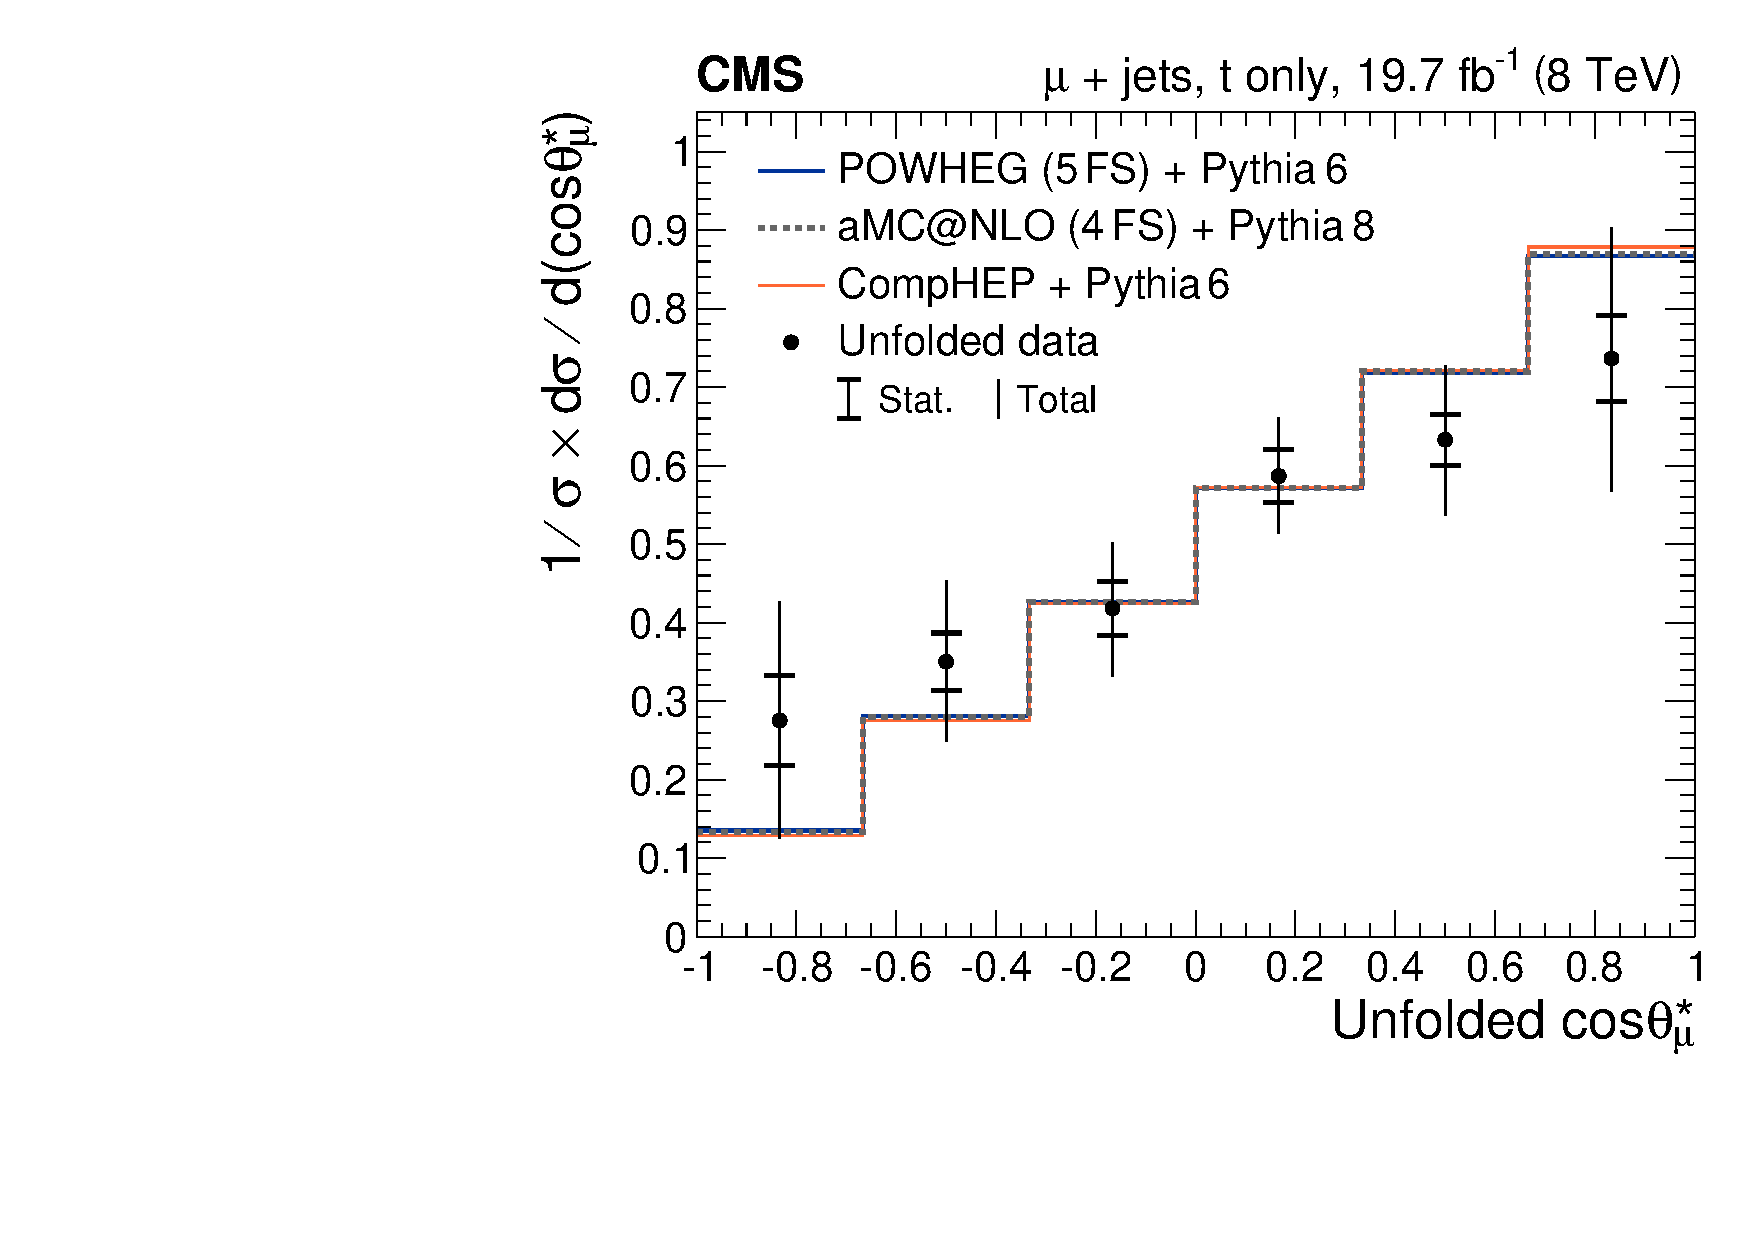
\includegraphics[width=0.48\textwidth]{figures/polarization/result/unfolded_mu_top.pdf}}
\hspace{0.02\textwidth}
\subfloat[]{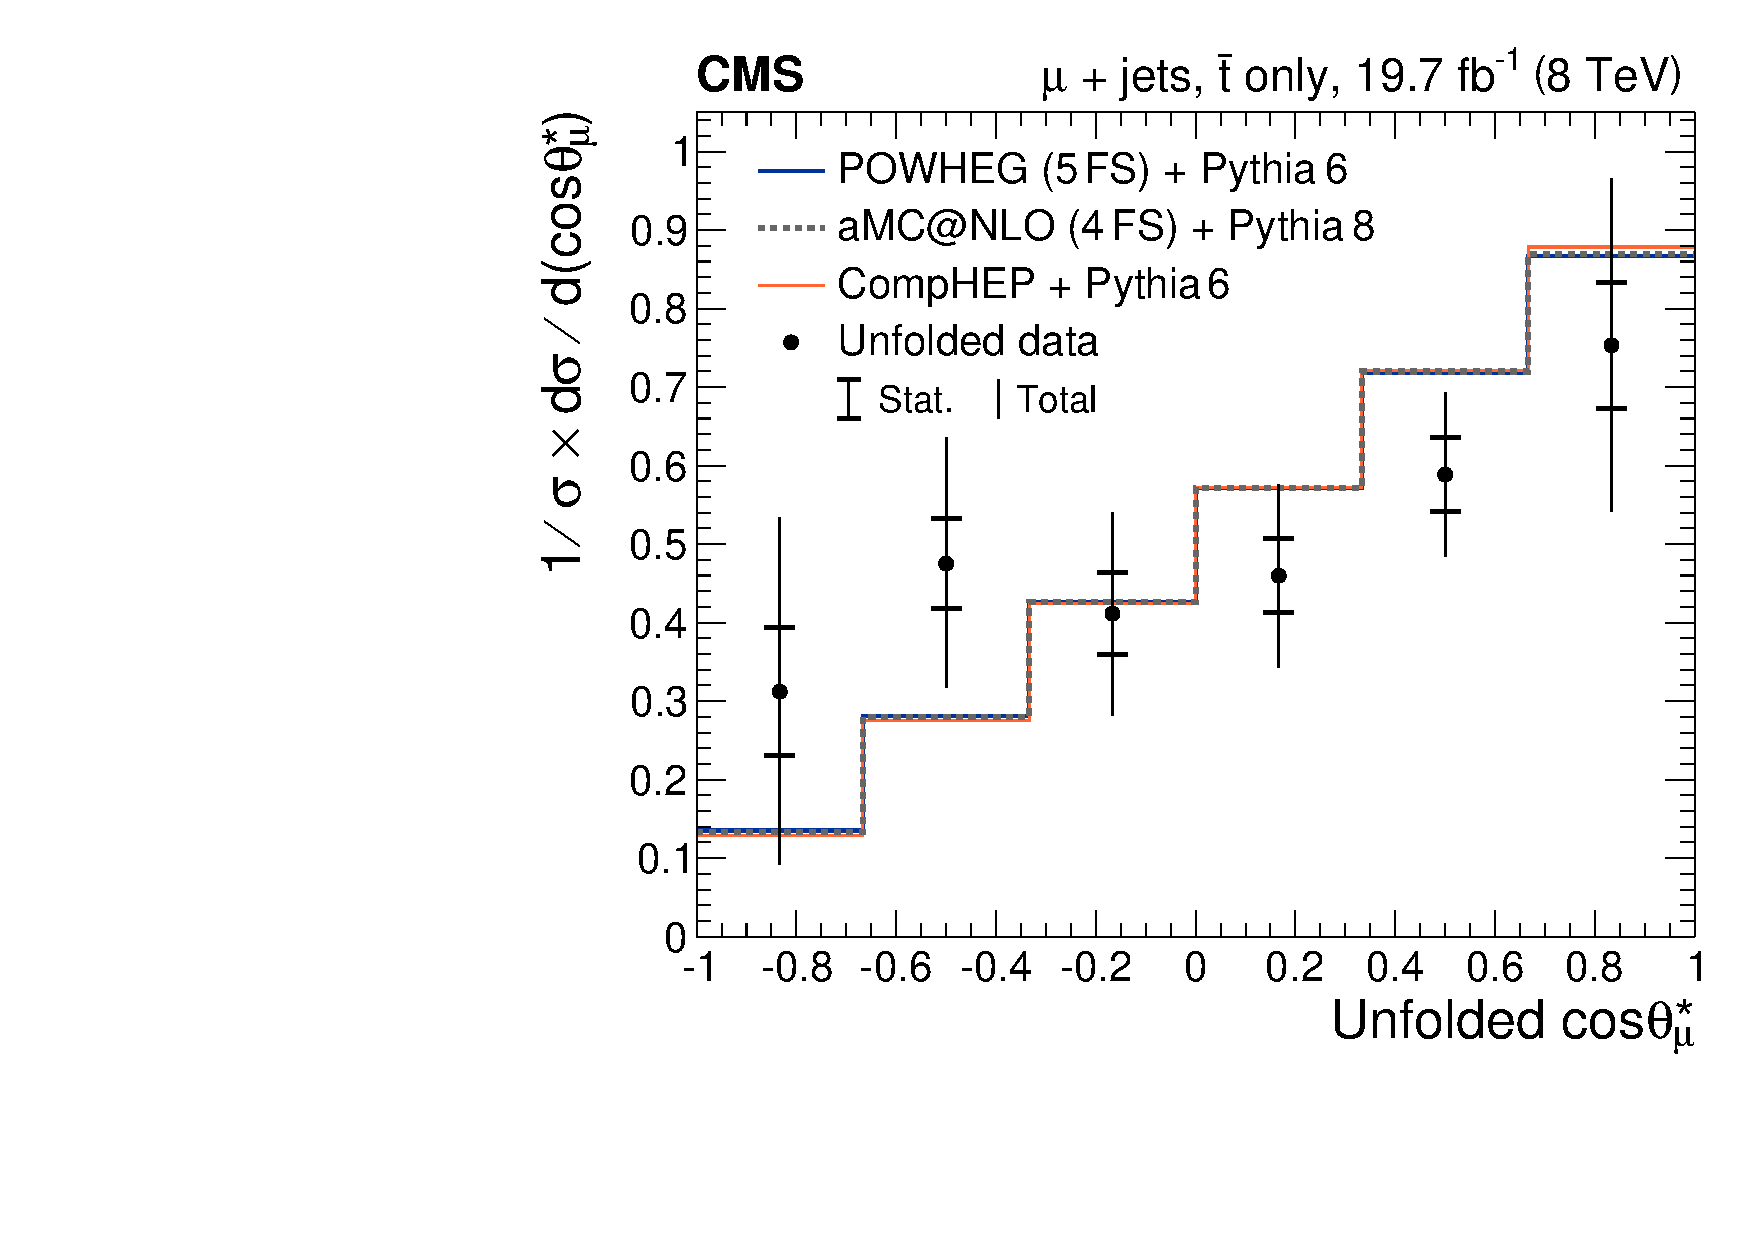
\includegraphics[width=0.48\textwidth]{figures/polarization/result/unfolded_mu_antitop.pdf}}\\
\subfloat[]{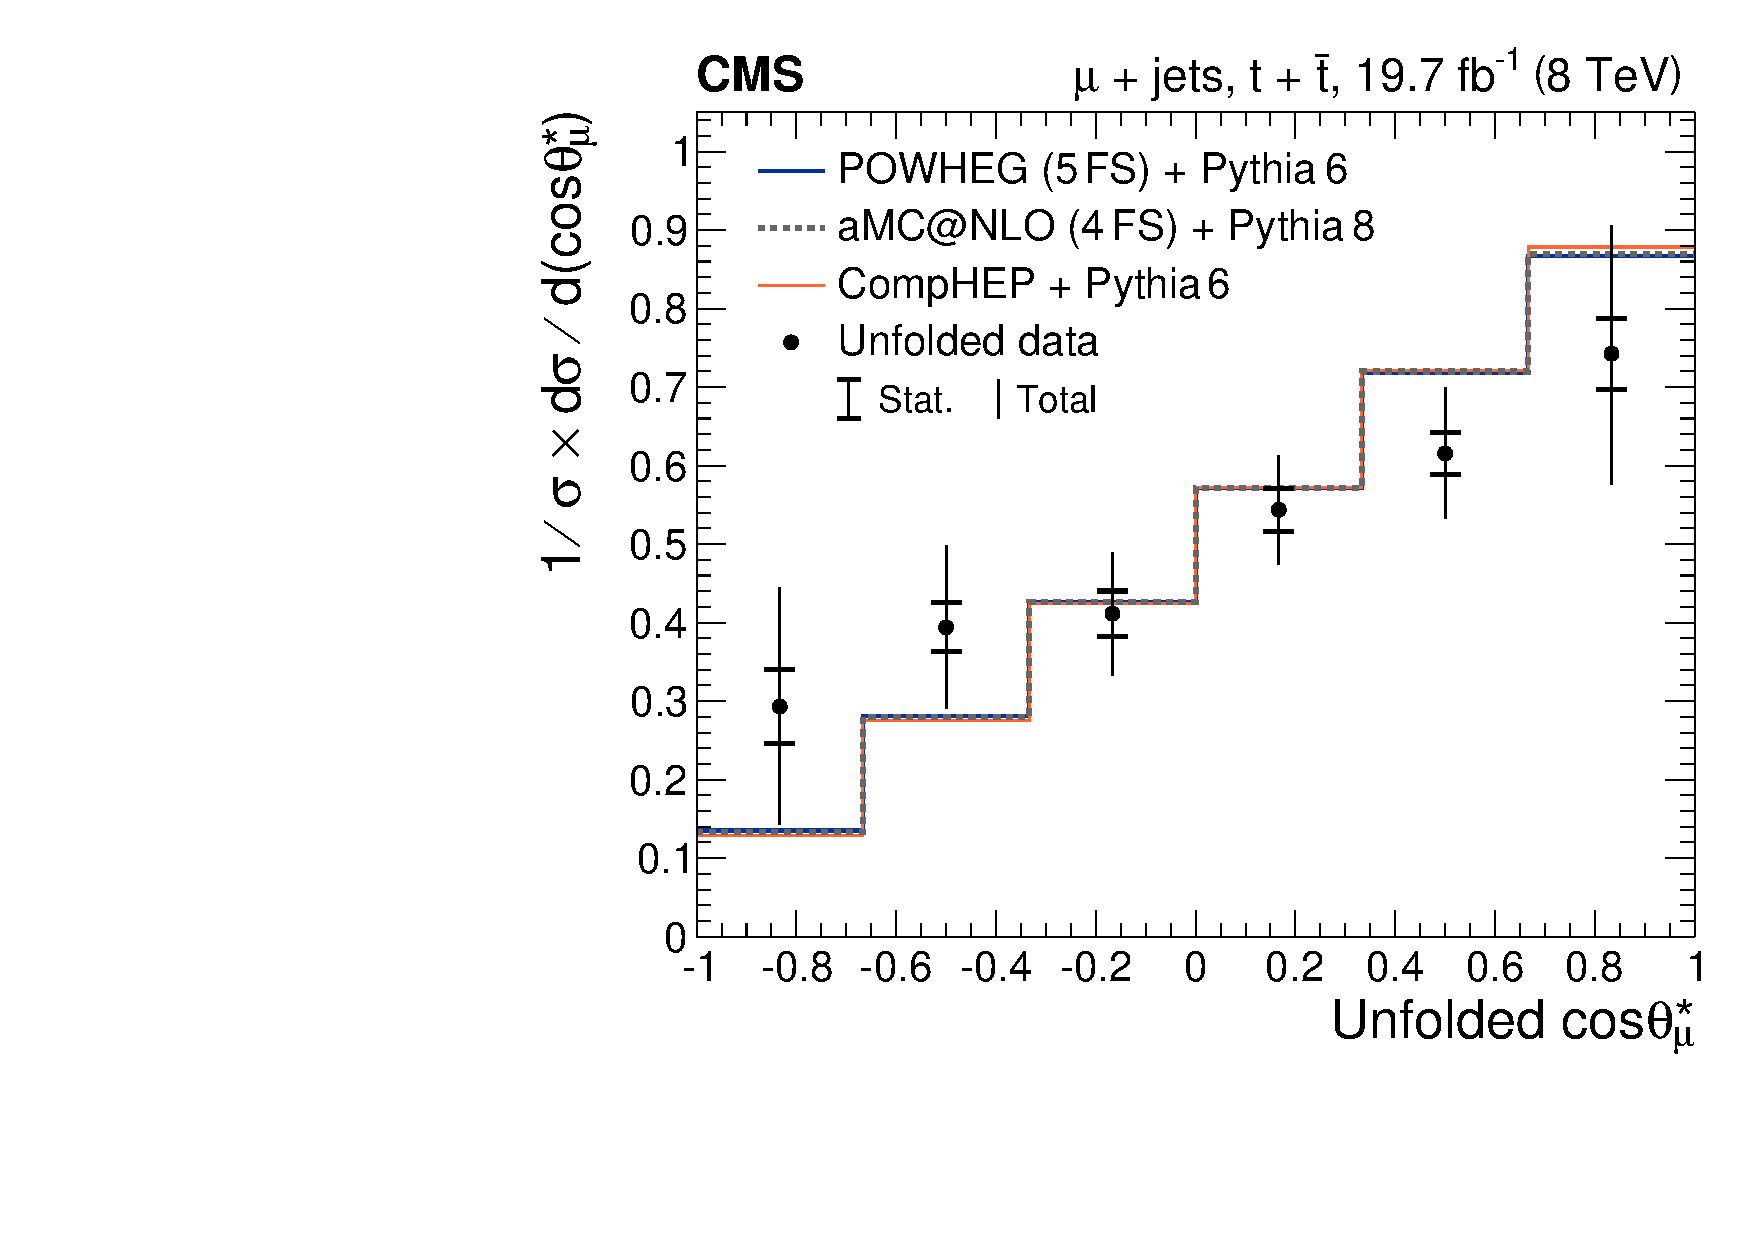
\includegraphics[width=0.48\textwidth]{figures/polarization/result/unfolded_mu.pdf}}
}


\newcommand{\AlResultCombined}{\ensuremath{\Big[26.0\pm 10.5 \Big]\cdot 10^{-2}}\xspace}
\newcommand{\AlResultCombinedStatSys}{\ensuremath{\Big[26.0\pm 2.6 \mathrm{(stat.)}\pm 10.2\mathrm{(syst.)} \Big] \cdot 10^{-2}} \xspace}
\newcommand{\AlResultCombinedPvalue}{\ensuremath{4.6\cdot 10^{-2}}\xspace}

\newcommand{\AlResultTop}{\ensuremath{\Big[29.0\pm 10.5 \Big]\cdot 10^{-2}}\xspace}
\newcommand{\AlResultTopStatSys}{\ensuremath{\Big[29.0 \pm 3.2 \mathrm{(stat.)} \pm 10.0\mathrm{(syst.)} \Big]\cdot 10^{-2}}\xspace}
\newcommand{\AlResultTopPvalue}{\ensuremath{7.9\cdot 10^{-2}}\xspace}

\newcommand{\AlResultAntiTop}{\ensuremath{\Big[21.1\pm 13.8 \Big]\cdot 10^{-2}}\xspace}
\newcommand{\AlResultAntiTopStatSys}{\ensuremath{\Big[21.1\pm 4.6\mathrm{(stat.)}\pm 12.6\mathrm{(syst.)} \Big]\cdot 10^{-2}}\xspace}
\newcommand{\AlResultAntiTopPvalue}{\ensuremath{5.0\cdot 10^{-2}}\xspace}


From data, we measure

\begin{align}
\AmuT          & = \AlResultTopStatSys = \AlResultTop , \\
\AmuTbar       & = \AlResultAntiTopStatSys = \AlResultAntiTop , \\
\AmuTplusTbar & = \AlResultCombinedStatSys = \AlResultCombined
\end{align}

using TUnfold. The measured asymmetries are compatible with a p-value of

\begin{align}
\AmuT:&\hspace{0.3cm} p(\mathrm{data |SM})          = \AlResultTopPvalue , \\
\AmuTbar:&\hspace{0.3cm} p(\mathrm{data |SM})      = \AlResultAntiTopPvalue , \\
\AmuTplusTbar:&\hspace{0.3cm} p(\mathrm{data |SM}) = \AlResultCombinedPvalue
\end{align}

with the SM value of $43.8\cdot 10^{-2}$ as predicted by \POWHEG.



\begin{align}
\AmuT          & = \Big[31.7\pm 3.7 \mathrm{(stat.)}\pm 10.9\mathrm{(syst.)} \Big]\cdot 10^{-2} = \Big[31.7\pm 11.2 \Big]\cdot 10^{-2} , \\
\AmuTbar       & = \Big[20.3\pm 5.7 \mathrm{(stat.)}\pm 15.0\mathrm{(syst.)} \Big]\cdot 10^{-2} = \Big[20.3\pm 16.0 \Big]\cdot 10^{-2} , \\
\AmuTplusTbar & = \Big[27.6\pm 3.1 \mathrm{(stat.)}\pm 11.1\mathrm{(syst.)} \Big]\cdot 10^{-2} = \Big[27.6\pm 11.5 \Big]\cdot 10^{-2} 
\end{align}

using the 2-bin analytic unfolding method as cross check.



%##############################################
\section{Limits on anomalous couplings}
%##############################################

topfit

combine: t-channel 8TeV~\cite{Khachatryan:2014iya}, Whelicity at 8TeV~\cite{Khachatryan:2016fky}


\myfigure{\label{fig:polarization-limits}sdfs dgfsdfg dfgdfg dsfgdfg sdfg sdfg dsfgdsf gsdf gsd fgdsfgsd fgds fg dsfg d sgfg dsfg dsf gdsf gdsf gsdfg sdfgds fg}{
\subfloat[]{\adjincludegraphics[height=4.55cm,trim={0 0 {0.195\width} 0},clip]{figures/polarization/limits/Ptvl-nol.pdf}}
\hspace{0.02\textwidth}
\subfloat[]{\adjincludegraphics[height=4.55cm,trim={0 0 {0.0\width} 0},clip]{figures/polarization/limits/Ptvr.pdf}}\\
\subfloat[]{\adjincludegraphics[height=4.55cm,trim={0 0 {0.195\width} 0},clip]{figures/polarization/limits/Ptgl-nol.pdf}}
\hspace{0.02\textwidth}
\subfloat[]{\adjincludegraphics[height=4.55cm,trim={0 0 {0.0\width} 0},clip]{figures/polarization/limits/Ptgr.pdf}}
}
